%%%%%%%%%%%%%%%%%%%%%%%%%%%%%%%%%%%%%%%%%%%%%%%%%%%%%%%%%%%%%%%%%%%%%%%%%%%%%%%%
\Chapter{Literature Overview}{}{}
\label{ch:related-work}
%%%%%%%%%%%%%%%%%%%%%%%%%%%%%%%%%%%%%%%%%%%%%%%%%%%%%%%%%%%%%%%%%%%%%%%%%%%%%%%%
% 
In this chapter, we give a literature overview of the state of the art that is
relevant for this thesis. We start with a brief literature summary with regards
to (electrical) flows. Note that we will discuss (electrical) flows formally in
more detail in~\cref{ch:foundations}. For now it suffices that an electrical
flow represents some physical flow that differs from a graph-theoretical flow in
the sense that it has some (roughly speaking) balancing properties that makes it
inefficient in most cases with regards to optimization criteria that we focus on
(\eg, maximizing the throughput). However, it reduces the overall energy loss
(see~\cref{ch:network-analyzes:eq:minimize-losses-quadratic-eq}) making it more
energy efficient. In addition, there are different approximation levels for
electrical flows that are used for certain scenarios, which we discuss in more
detail in~\cref{ch:foundations}. A common way to calculate electrical flows is
by using solvers that search for a feasible solution. However, this gives us
very little structural insights in how electrical flows work and thus, we give
an overview of common reduction and transformation rules from the literature
in~\cref{ch:related-work:sec:analyses} that make use of the superposition
principle for linear systems. Note that we use the term network analysis in the
context of calculating an electrical flow by using techniques that give more
insights into the problem structure.
% 
There is currently not much known about structural insights to solve electrical
flows using algorithms. We only found reduction and transformation rules that are
not much investigated for a more complex power grid analysis. The only problem
specific algorithm known is an exponential time
algorithm~\parencite{Ses61,Sha87}. 

A major contribution of this work are placement problems. Placement problems
exploit the structure in the sense that they modify the electrical flow such
that some objective is optimized such as the throughput. This optimization is
possible since the electrical flow has the property of balancing itself and
thus, does not represent the best possible flow for a given topology. A
literature overview on the behavior of electrical flows and the placement
problems we focus on is given in~\cref{ch:related-work:sec:braess-paradox}. For
the placement problems, we distinguish between discrete
(see~\cref{ch:related-work:sec:switching}) and continuous placement problems
(see~\cref{ch:related-work:sec:facts}), on which we give literature overviews by
considering the placement of switches and~\acrlong{facts} (\gls{facts}),
respectively. For transmission network expansion planning, we will focus on
literature for the wind farm planning with the focus on wind farm cabling
in~\cref{ch:related-work:sec:wind-farm-cabling}. In this literature overview, we
will see that there is little known about the problem with regards to structural
results. Since there are not a lot of structural results, there are not a lot of
algorithms to tackle electrical flows and because of that to tackle the
aforementioned placement problems using algorithms.
% 
%%%%%%%%%%%%%%%%%%%%%%%%%%%%%%%%%%%%%%%%%%%%%%%%%%%%%%%%%%%%%%%%%%%%%%%%%%%%%%%%
\section{Graph-theoretical Flows and Electrical Flows}
\label{ch:related-work:sec:gt-flows-power-flows}
%%%%%%%%%%%%%%%%%%%%%%%%%%%%%%%%%%%%%%%%%%%%%%%%%%%%%%%%%%%%%%%%%%%%%%%%%%%%%%%% 
% 
The graph-theoretical flow complies with the conservation of flow meaning that
the incoming flow is equal to the outgoing flow. This is similar to the
principle of conservation of energy. If maximized it is called~\acrlong{mfp}
(\gls{mfp};
\cref{ch:foundations:sec:graph-theoretical-flows:para:maximum-flow-problem}). If
each edge has a cost function, the problem of minimizing the total cost is
called~\acrlong{mcfp} (\gls{mcfp};
\cref{ch:foundations:sec:graph-theoretical-flows:para:minimum-cost-flow-problem}).
Both optimization variants are well known problems with efficient algorithms for
both~\gls{mfp}~\parencite{Gol14}
and~\gls{mcfp}~\parencite{Gol89,Edm72,Kle67,Orl97,Gol90}. The graph-theoretical
flow complies with the conservation of flow (\ie, incoming is equivalent to the
outgoing flow at each vertex) and the capacity constraints at each edge.
However, electrical flows that we also call \emph{power flows} have to obey some
physical laws. The physical relationship between current, voltage, and
resistance was first formalized by~\textcite{Kir47} in~\acrlong{kvl} (\gls{kvl})
and \acrlong{kcl} (\gls{kcl}). The latter is equivalent to the flow conservation
of graph-theoretical flows. The~\gls{kvl} represents a conservation of flow on
cycles and not on vertices. The latter law states that the flows in a cycle
(also known as mesh) sum up to zero. A base is a maximum independent set.
\citeauthor{Kir47} introduces for the~\gls{kvl} the concept of cycle bases,
which we will discuss in more detail in~\cref{ch:network-analysis}. He shows
which equations form a cycle base (\ie, a number of equations that suffice to
compute the~\gls{kvl}), and he reformulates the voltage law in terms of a cycle
base. This basically means that the number of equations for the~\gls{kvl} is
reduced from potentially exponentially many equations to polynomially many
equations while assuming simple graphs. Later, \textcite{Max65} describes the
electrical charge, electrical current, electrical field and magnetic field in
more detail. These works formalize the operation of power grids and thus, build
the foundation that is used in the power flow literature.
 
\paragraph{(Optimal) Electrical Flow Solution Techniques} 
% 
In the aforementioned paragraph, we described that an electrical flow complies
with the~\gls{kcl} and~\gls{kvl}. These laws constrain the electrical flow. A
usual question in power grids is if the demand can be fulfilled with the
currently available generation. This problem is called~\acrlong{feas}
(\gls{feas}). If we constraint the flow with the~\gls{kcl} and~\gls{kvl} law, we
call it the electrical flow feasibility problem. We will see
in~\cref{ch:foundations:sec:power-flow-analyses} that there are different
approximations for electrical flow and thus, different feasibility problems. In
the following, we will give a brief overview of existing solution techniques for
electrical flow feasibility problems in general. We will also mention the
\acrlong{opfp} (\gls{opfp}) that is an optimization problem that minimizes the
generation costs while complying with an electrical flow (here called power
flow).

There are different techniques to solve electrical flow feasibility problems.
One of the first surveys outlines digital techniques to solve the electrical
flow~\parencite{Sas67}. Another survey of electrical flow and optimal electrical
flow solution techniques is given by~\textcite{Huneault1991} outlining the first
automated digital solution technique by~\textcite{War56}, and the Gauss-Seidel
method introduced by~\citeauthor{Car62}~\parencite{Car62,Car79}, that is later
replaced by the Newton-Raphson method~\parencite{Pes68,Cos99}.
% 
% \citeauthor{Car62} also
% introduced the first~\acrlong{opf} (\gls{opf}) formulation.

The problem of generating the required amount of power while obtaining minimum
operation cost is called \emph{\acrlong{edp}} (\gls{edp}).
% 
% For the classical~\gls{edp} a integer non-linear program
% needs to be solved, which is~\NP-hard~\parencite{Jue10b}. 
% 
To cope with the~\gls{edp} while incorporating an electrical flow feasibility
problem is called the~\acrlong{opfp} (\gls{opfp}) that was introduced
by~\textcite{Car62}. The development of solution techniques on~\gls{opfp} is
summarized by~\textcite{SurveyOPF1,SurveyOPF2}.

\textcite{Sto74} reduces the memory consumption and running time for electrical
flow feasibility problems by introducing sparsity techniques for the admittance
matrix and compares it to other methods. The idea behind the approach
of~\citeauthor{Sto74} is that the power grid has a very sparse network
structure~\parencite[p.17]{Cai12} and thus, techniques that exploit the sparsity
improve the running time and memory consumption. A comparison of different power
formulations (see~\cref{ch:foundations:sec:power-flow-analyses:subsec:AC-Model})
is given by~\textcite{Cos08}. \textcite{Mol19} give a survey of relaxations and
approximations of the electrical flow equations.
In~\cref{ch:related-work:sec:analyses}, we outline some literature that mention
possible ways to analyze power grids. Note that as far as we know there is no
\textquote{purely} algorithmical approach to solve the power flow problem apart
from an exponential time algorithm~\parencite{Ses61,Sha87}. For linear systems
there are reduction and transformation rules known, which are not used so far to
create an algorithm for electrical flows. A literature overview including known
applications of these rules is given in the following.
% 
% The first method used for the AC load flow analyses was the also the
% Gauss-Seidel method.
% 
% - slow because of slow convergence~\parencite[p. 71]{wood1996power}
% - difficulties with negative reactance branches
% - each bus is treated independently
% -> each correction to one bus requires changes to the other buses
% 
% Another possibility to solve the problem is the newton-raphson method 
% based on the idea to calculate the correction (take all interactions into
% account) [reformulate]
% 
% Afterwards 
% - 1929 pf solved with analog network analyzern
% - Lagrangian techniques for the optimality cond. but neglegts variable bounds 
% (Squires 61)
% - Carpentier - optimality conditions for the OPF incl. variable bounds 
% (Kuhn-Tucker-Conditions) + first fully formulated OPF
% 
%%%%%%%%%%%%%%%%%%%%%%%%%%%%%%%%%%%%%%%%%%%%%%%%%%%%%%%%%%%%%%%%%%%%%%%%%%%%%%%%
\section{Reduction Rules for the Analysis of Power Grids}
\label{ch:related-work:sec:analyses}
%%%%%%%%%%%%%%%%%%%%%%%%%%%%%%%%%%%%%%%%%%%%%%%%%%%%%%%%%%%%%%%%%%%%%%%%%%%%%%%%
% 
\begin{figure}
    % 
    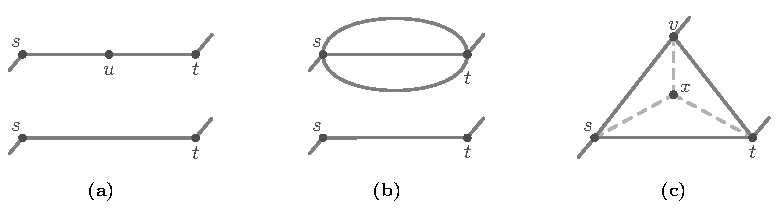
\includegraphics{relatedwork/figures/transformation.pdf}
    % 
    \caption[Common network reduction rules.]{Three different
    subgraphs that lead to different transformation rules each. These common
    transformation rules provide possibilities to reduce the network size. (a)
    In a series contraction a path with vertices of degree two can be contracted
    to a single edge. (b) In a parallel contraction multiple parallel edges can
    be contracted to a single edge. (c) The~\glssymbol{deltawye}-transformation
    (\glslongform{deltawye}; respectively \glssymbol{wyedelta}-transformation
    known as~\glslongform{wyedelta}) represent a possibility to increase
    (respectively decrease) the number of vertices and reduce (respectively
    increase) the number of triangles by one.
    % 
    }
    % 
    \label{ch:realted-work:fig:transformation}
\end{figure}
% 
In this work, we focus on a linear approximation of the electrical flow. Thus,
all equations, constraints, and objectives are linear functions. The goal of the
network analysis is to design algorithms that exploit the structure of the
problem such that these algorithms run in polynomial time in the input size.
There are different possibilities to analyze power grids. The common way to
compute electrical flows is to solve a set of linear equations using solvers
such as the~\gls{gurobi}~\parencite{online:Gurobi,gurobi}. However, the input
size has often a big influence on the running time to solve a problem. A
possibility to reduce the input size is to use reduction rules. However,
reduction rules in power grids include contraction and transformation rules.
Contraction rules are series
(see~\cref{ch:realted-work:fig:transformation}\screen{a}) and parallel
contractions (see~\cref{ch:realted-work:fig:transformation}\screen{b}) and
transformation rules are~\glssymbol{deltawye}- (\glslongform{deltawye}) and
\glssymbol{wyedelta}- (\glslongform{wyedelta}) transformations
(see~\cref{ch:realted-work:fig:transformation}\screen{c}). The latter rule
transforms a triangle to a star by adding one vertex into the center and adding
edges from the center to the already existing vertices, while removing the
original edges, and vice versa for the inverse transformation, respectively. The
generalization of the \glssymbol{deltawye}-
and~\glssymbol{wyedelta}-transformations are the star-mesh- (or star-polygon-)
transformations~\parencite{Lie73,Bed61}. Other common rules are self-loop and
degree-1 removals.

These reduction rules are applied on different problems in different fields of
research such as in statistical physics involving the evolution of crystal
lattice energy~\parencite{Bax16}, network
reliability~\parencite{Leh63,Sat93,Tra02}, knot theory~\parencite{Rei83,Tra02},
and graph theory~\parencite{Ake60,Cha17}. We start with some initial algorithmic
results on the transformation rules in the following.

\paragraph{Reducibility of Graphs and Complexity of Reduction Algorithms}
% 
The first more general structural observations concerning reduction rules are
by~\textcite{Ake60} and~\textcite{Leh63}. Both independently introduce the
conjecture that by using a combination of~\glssymbol{wyedelta}-
and~\glssymbol{deltawye}-transformations, as well as series and parallel
contractions the connected, two-terminal, undirected, planar graph can be
reduced to a single edge connecting the given
terminals~\parencite[pp.795ff.]{Leh63}. The latter conjecture is then
independently proven by~\textcite{Gru03} using a graph without terminals, and a
complicated and non-constructive proof by~\textcite{Epi66}.
Using~\glssymbol{deltawye}-
and~\glssymbol{wyedelta}-transformations~\citeauthor{Epi66} proves that any
polyhedral graph (\ie, an undirected graph that is a representation of a convex
polyhedron) can be reduced to a~$K_4$ (\ie, complete graph with four vertices).
The proofs of the conjecture is simplified by~\textcite{Tru89} using a
constructive proof incorporating graph minors. One major property used
in~\citeauthor{Tru89}'s proof is that planar graphs can be embedded as grid
graphs. \citeauthor{Tru89} provides a much simpler polynomial time algorithm for
planar graphs than the one by~\textcite{Feo85}.
\citeauthor{Tru89}'s~\parencite{Tru89} algorithm
requires~$\bigO(\fmagnitude{\glssymbol{vertices}}^2)$ space, but he did not
mentioned the running time of the algorithm. However, \textcite{Feo85} designed
a more complex algorithm that runs
in~$\bigO(\fmagnitude{\glssymbol{vertices}}^2)$ time and
needs~$\bigO(\fmagnitude{\glssymbol{vertices}})$ space. \textcite{Val79} showed
that the series, parallel, loop, and single degree reductions for
series-parallel-graphs can be done in~$\bigO(\fmagnitude{\glssymbol{vertices}})$
time. In addition, \textcite{Pol83} showed that every~\gls{wyedeltagraph} (\ie,
a graph that can be reduced to a vertex by the aforementioned reduction rules)
is planar. The term~$C_i$ (also known as~$i$-cyclic graph) represents a closed
walk of length~$i\in\naturals$ with~$i$ being the number of vertices. A planar
graph is a~\gls{wyedeltagraph} if and only if it is a~$(C_5+2K_1, K_2\times
C_4)$-free graph~\parencite{Pol83} or~$(K_5, K_{2,2,2}, C_8(1,4), K_2\times
C_5)$-free graph~\parencite{Arn90,Sat90}, respectively. To the extent of our
knowledge, it is unknown whether these algorithms are applicable to power grids
or not. Some application to graph-theoretical problems are given in the next
paragraph.
% 
\paragraph{Preservation of Optimization Properties}
% 
Regardless of the structural point of view, these transformations are used when
solving algorithmic problems. 
% 
Dependent on the problem, it is necessary to show that the transformation and
contraction rules preserve a solution space. This is roughly done
by~\textcite{Ake60} for the~\acrlong{mfp} (\gls{mfp}) and~\acrlong{sppp}
(\gls{sppp}).
% 
He used the transformations to simplify the network such that algorithmic
problems become easier to solve. \textcite{Ake60} applied the transformations to
solve~\gls{sppp} and~\gls{mfp} on undirected~$2$- and~$3$-terminal graphs while
preserving the optimal length or flow value. Interestingly, the transformations
shown in~\textcite{Ake60} also behave dually meaning that, \eg, the calculation
of the capacities of the series reduction is the calculation of the parallel
reduction in the dual problem. The duality of the transformations is shown
for example in~\textcite{Ake60}. Another work by~\textcite{Cha17} uses these
reduction rules to untangle planar curves meaning to simplify a planar graph
with a certain number of self-crossings. In the next paragraph, we show the
usage of the reduction rules with regards to network reliability. Within network
reliability there is a lot of literature available that gives structural results
on the hardness of the problem and uses methodology to tackle~\NP-hard problems,
which we will use for some placement problems.
% 
\paragraph{Preservation of Network Reliability}
% 
In network reliability these reductions rules are used extensively. Network
reliability studies the probability that at least one path connecting two
terminals operates successfully. The edges in such a network have success
probabilities. The problem of computing the all-terminal reliability for
arbitrary networks is known to be~\NP-hard~\parencite{Pro83,Val79a}. The hardness
remains even for planar graphs~\parencite{Ver05}. 
% 
% Application of the all-terminal reliability are given
% in~\parencite{Pol83,Pol90,Arn90,el1990two}
% \franzi{check again}. 
% 
\textcite{Leh63} showed that series, parallel, degree-1, and loop reductions
preserve reliability in the two-terminal and undirected network case. The
\glssymbol{deltawye}- and \glssymbol{wyedelta}-transformations for boolean functions
(also known as switching-functions) are introduced by~\textcite[Section
4]{Leh63}. However, he shows that these transformations do not calculate the
exact probability, but an approximation to it.
% 
% He used numerical transformation tables since the values were between~$0$
% and~$1$. 
% 
Since the problem is in general~\NP-hard, \textcite{Sat93} developed efficient
algorithms for special graph classes, which run
in~$\bigO(\fmagnitude{\glssymbol{vertices}}\log\fmagnitude{\glssymbol{vertices}})$
time.
% 
% , where~\glssymbol{vertices} represents the set of buses. 
% 
The latter work~\parencite{Sat93} uses the technique of forbidden minors (\ie, a
minor~\minor is a graph that can be extracted from a graph~\glssymbol{graph} by
applying vertex and edge deletions and edge contractions) to develop efficient
algorithms for reliability analysis on graph subclasses. \citeauthor{Sat93} not
only focused on the two terminal case, but on the $K$-terminal reliability that
focuses on the probability that there is a path between every pair of terminals.
Where~\textcite{Leh63} showed that not all transformations are reliability
preserving reductions, \textcite{Sat93} focused on reliability preserving
reductions and introduced a
\gls{trisubgraph}-Y-reduction. They focused on block-cut-trees, $3$-connected
graphs, and series-parallel graphs. For the latter graph structure they observed
that it depends on the distribution of the terminals whether the graph is
reducible or irreducible and thus, reliability preserving using the standard
reduction rules or not. The $K$-terminal reliability on
series-parallel-reducible networks can be computed
in~$\bigO(\fmagnitude{\glssymbol{edges}})$ time using series, parallel,
degree-1, and -2 contractions~\parencite[pp.827ff.]{Sat85}. However, for
series-parallel-irreducible graphs these reduction rules are not sufficient and
thus, \textcite{Sat85} designed a linear time algorithm using
the~\emph{polygon-to-chain reduction} that reduces two parallel
paths~$\fpath{1}{\source}{\sink}$ and~$\fpath{2}{\source}{\sink}$ with inner
vertices of degree-2 to one path having a length of $\max\{
\fmagnitude{\fpath{1}{\source}{\sink}},
\fmagnitude{\fpath{2}{\source}{\sink}} \}$. For basically series-parallel
directed graphs (\ie, graphs where the underlying graph is a series-parallel
graph)~\textcite{Agr84,Agr85} provide an $\bigO(\fmagnitude{\glssymbol{edges}})$
time algorithm to compute source-to-K-terminal reliability.
\textcite{Pol86,Pol90} show that for~$K_2\times C_4$-free graphs the reliability
can be computed in linear time and~\textcite{Pol92} show that the all-terminal
reliability of a~$(K_5, K_ {2,2,2})$-free graph can be computed
in~$\bigO(\fmagnitude{\glssymbol{vertices}}\log\fmagnitude{\glssymbol{vertices}})$
time. \textcite[p.13; Proposition~2]{Sat93} show that a~\gls{wyedeltagraph}
allows a~\gls{trisubgraph}-Y reduction resulting in a~\gls{wyedeltagraph}.

\paragraph{Further Results}
% 
There are results on reducibility for planar graphs, non-planar graphs, and
special graphs that we outline here. \textcite{Git91} proofs for reducibility
for graphs with no~$K_5$ minor and graphs with no~$K_{3,3}$ minor. The
reducibility for projective-planar graphs (\ie, a projective plane is an
extension of the euclidean space, where parallel edges intersect in a point and
thus, all edges intersect in some point) and graphs with crossing number one was
shown by~\textcite{Arc00}. For 4-terminal reducibility of planar graphs,
\textcite{Demasi:2015:FTP:2722129.2722244} show that a sufficiently
connected~\gls{cubicgraph} (\ie, a graph, where all vertices have a degree of
three) are reducible if and only if it does not contain a Petersen graph as
minor. Later \textcite{Wag15} presents a reducibility for almost-planar graphs
with the condition that all graphs in the reduction sequence remain
almost-planar. Other works define the reducibility with a set of forbidden
minors~\parencite{DBLP:journals/jgt/Yu04a,DBLP:journals/combinatorics/Yu06} and
design algorithm for 3-terminals, special cases of 4-terminal planar graphs,
$k$-cofacial terminals in planar graphs~\parencite{Git91,doi:10.1002/net.20399}.
% 
% \franzi{Read the work of~\citet{6316101} and incorporate it}
% 
%%%%%%%%%%%%%%%%%%%%%%%%%%%%%%%%%%%%%%%%%%%%%%%%%%%%%%%%%%%%%%%%%%%%%%%%%%%%%%%
% \begin{landscape}
%     \begin{table}
%         % 
%         % latex table generated in R 3.2.2 by xtable 1.8-0 package
% Wed Jan 27 11:17:04 2016
{\setlength{\tabcolsep}{0.3em}}
{\renewcommand{\arraystretch}{1}}% for the vertical padding
\small
% \begin{tabular}{p{2cm}p{3cm}p{3cm}p{3cm}p{3cm}p{3cm}}
\begin{tabular}{%
>{\centering\arraybackslash}m{3cm}%
>{\arraybackslash}m{2.5cm}%
>{\centering\arraybackslash}m{2cm}%
>{\arraybackslash}m{3.5cm}%
% >{\centering\arraybackslash}m{2cm}%
>{\arraybackslash}m{2cm}%
% >{\centering\arraybackslash}m{0.56cm}%
% >{\arraybackslash}m{2.3cm}%
% >{\centering\arraybackslash}m{0.56cm}%
% >{\arraybackslash}m{1.5cm}%
% >{\centering\arraybackslash}m{0.56cm}%
}%
% 
\toprule
  \multirow[c]{1}*{Graph Structure}     & 
  \multicolumn{1}{c}{Problem}           &
  \multicolumn{1}{c}{Complexity}        & 
  \multicolumn{1}{c}{Reduction Rules}   &
  % \multicolumn{1}{c}{Algorithm}         &
  \multicolumn{1}{c}{Cite}
  \\
%-------------------------------------------------------------------------------
%-------------------------------------------------------------------------------
% 
%-------------------------------------------------------------------------------
%-------------------------------------------------------------------------------
% 
%-------------------------------------------------------------------------------
%-------------------------------------------------------------------------------
 \midrule  
%-------------------------------------------------------------------------------
%-------------------------------------------------------------------------------
\rowcolor{Table-Line-Marker}
% 
    Arbitrary graphs 
    & All-terminal reliability 
    & \NP-hard 
    & -- 
    % & -- 
    & \parencite{Pro83,Sat90}
\\
    Planar graphs 
    & Reliability $R(\glssymbol{graph})$ 
    & \NP-hard 
    & -- 
    % & -- 
    & \parencite{Ver05} 
\\
\rowcolor{Table-Line-Marker}
% 
\rowcolor{Table-Line-Marker}
    Series-parallel reducible graph 
    & K-terminal reliability $R_K(\glssymbol{graph})$ 
    & $\bigO(\fmagnitude{\glssymbol{edges}})$ 
    & 
    \begin{tabular}[c]{@{}l@{}}
    Series, 
    \\ parallel, and 
    \\ degree-1
    \end{tabular} 
    % & -- 
    & -- 
\\
    Series-parallel irreducible graph 
    & K-terminal reliability $R_K(\glssymbol{graph})$ 
    & linear time 
    & 
    \begin{tabular}[c]{@{}l@{}}
        Polygone-to-chain, 
        \\ series, 
        \\ parallel, and 
        \\ degree-1
    \end{tabular} 
    % & -- 
    & \parencite{Sat85} 
\\
\rowcolor{Table-Line-Marker}
    Basically series-parallel digraph 
    & Source-to-K reliability
    & $\bigO(\fmagnitude{\glssymbol{edges}})$ 
    & -- 
    % & -- 
    & \parencite{Agr85} 
\\
    $K_2\times C_4$-free graph 
    & Reliability $R(\glssymbol{graph})$ 
    & linear time 
    & -- 
    % & -- 
    & \parencite{Pol83,Pol86} 
\\
% 
\rowcolor{Table-Line-Marker}
    $\Delta-Y$-graph 
    & Reliability~$R(\glssymbol{graph})$ 
    & $\bigO(\fmagnitude{\glssymbol{vertices}}^2)$ 
    & -- 
    % & -- 
    &  
\\
% 
    $(K_5,K_{2,2,2})$-free graph 
    & All-terminal reliability 
    & $\bigO(\fmagnitude{\glssymbol{vertices}}\log
    \fmagnitude{\glssymbol{vertices}})$
    & -- 
    % & -- 
    & \parencite{Pol92} 
\\
%--------------------------------------------------------------------------------------------------------------------------------------------------------------------------------------------------------------------------------------------------------------------
   \bottomrule
\end{tabular}%

%         % 
%         \caption[Overview of the results that make use of reduction rules.]
%         {Overview of the results that make use of reduction rules. This table
%         shows that different graph structures lead to different complexities.}
%         % 
%         \label{ch:switching:sec:complexity:tbl:complexity-overview}
%         % 
%     \end{table}
% \end{landscape}
%%%%%%%%%%%%%%%%%%%%%%%%%%%%%%%%%%%%%%%%%%%%%%%%%%%%%%%%%%%%%%%%%%%%%%%%%%%%%%%
% 
%%%%%%%%%%%%%%%%%%%%%%%%%%%%%%%%%%%%%%%%%%%%%%%%%%%%%%%%%%%%%%%%%%%%%%%%%%%%%%%%
\section{Braess's Paradox -- Effects that Influence the Power Grid Efficiency
and Stability}
\label{ch:related-work:sec:braess-paradox}
%%%%%%%%%%%%%%%%%%%%%%%%%%%%%%%%%%%%%%%%%%%%%%%%%%%%%%%%%%%%%%%%%%%%%%%%%%%%%%%%
% 
The main focus of this thesis is on placement problems with additional physical
properties. In the introduction (see~\cref{ch:intro}), we discuss two strategies
to improve the power grid efficiency. In contrast to our intuition, not only the
expansion of the power grid (\gls{tnep}; \cref{ch:intro:strategy:1}
in~\cref{ch:intro}), but also switching can be used to improve the efficiency of
the power grid. This implies that adding a new line to the power grid can also
decrease the throughput of the power grid or increase the overall generation
costs.

A similar phenomenon exists for road networks and is called Braess's
para\-dox \parencite{Bra68,Bra05}. Introducing a new road to the traffic network
might cause longer travel times~\parencite{You08}. The main reason is that every
participant wants to independently minimize its own travel time, while ignoring
the decision's effect on other travelers~\parencite{Pas97}. In addition,
\textcite{Pas97} show that the occurrence of the Braess's paradox highly depends
on the instance parameters, \ie, demand and congestion functions. Thus, the
paradox usually occurs within some bounds that make it possible that the network
might \textquote{grow in} and \textquote{grow out} of the paradoxical situation
with increasing (traffic) demand. 

\textcite{Coh91} describe the existence of the paradox in
mechanical~\parencite{Pet12} and electrical networks (for both
see~\parencite{Pen03}). Other works show that the paradox also appears in
oscillator networks~\parencite{Wit12}, where adding a line can cause
instabilities and even power outages, which confirms once more the existence of
the Braess's paradox in real power grids~\parencite[p.11]{Wit12}. Another
example for this exists in quantum physics~\parencite{Pal12}.

\textcite{Coh91} also emphasize the non-intuitive behavior of the Nash
equilibrium that arises in most physical networks. We know from~\textcite[p.4;
Section 3]{Dub86} that Nash Equilibria \textquote{tend to be inefficient in the
Pareto sense}. We will give an explanation of that
in~\cref{ch:network-analysis}. The Nash Equilibrium is a known fix point in Game
Theory and represents a state, where no player wants to change its choice. In
contrast, the Pareto optimum means that there is no possible better choice of
one player that does not decrease the payoff of another player. Thus, it is the
optimum with regards to a cost function. The Pareto front represents the set of
Pareto optima. However, the Pareto optimization plays a crucial role in the
multi-criteria optimization. We show an example for a Pareto front
in~\cref{ch:facts:sub:experiments-control-units:fig:plot-costs-losses}. An easy
example that shows Pareto optima and Nash Equilibriums is given
in~\textcite[p.5; Figures 2--4]{Dub86}.

Another theoretical insight given by~\textcite{Val06} explaining that the
Braess's paradox occurs very often in random graphs. Note that many of the
networks in the real world have properties similar to random
graphs~\parencite[p.xiii]{online:Hof19}. Thus, in~\cref{ch:switching}, we
exploit the Braess's paradox to improve the efficiency of the power grid,
whereas in the~\gls{tnep} problem, we have to add lines in a way that the
efficiency of the power grid increases and thus, the effect of the Braess's
paradox does not appear. The effect that the Braess's Paradox highly depends on
the instance parameters~\parencite{Pas97} is shown
in~\cref{ch:switching,ch:facts}, where we use switches and~\gls{facts} to
influence these parameters.
% 
%%%%%%%%%%%%%%%%%%%%%%%%%%%%%%%%%%%%%%%%%%%%%%%%%%%%%%%%%%%%%%%%%%%%%%%%%%%%%%%%
\subsection{Switching -- A Discrete Manipulation of the Power Grid Topology}
\label{ch:related-work:sec:switching}
%%%%%%%%%%%%%%%%%%%%%%%%%%%%%%%%%%%%%%%%%%%%%%%%%%%%%%%%%%%%%%%%%%%%%%%%%%%%%%%%
% 
Recall that switching is the process of temporarily removing a transmission line
from the power grid by using devices such as circuit breakers.
\citeauthor{Kir47} model this behavior by changing the resistance to
infinity~\parencite[p.501]{Kir47}.
% 
Switching was first analyzed as a negative effect in the power
grid~\parencite{GLAVITSCH198592} responsible for overloads, voltage drops, and
the loss of network stability.
%
\textcite{koglin1980overload} introduce transmission switching as a corrective
control action to reduce transmission line overloads. Later other positive
switching effects were recognized such as improving currents, decreasing loads
and angles, creating voltage drops, and changing the short-circuit
power~\parencite{GLAVITSCH198592,Hed11,744552}.

\textcite{1388507} and~\textcite{Fis08} introduce
the~\acrlong{otsp}~(\gls{otsp}) and its formulation based on
the~\acrlong{dcopf}~(\gls{dcopf})~\parencite{Cho06}, respectively.
The~\gls{otsp} using~\gls{dc}-constraints is called~\gls{dcots}.
\textcite{Fis08} observe that switching may improve the economic efficiency of
the~\acrlong{edp} (\gls{edp}). However, they could not find any general trend in
the physical characteristics of the switched lines.
%
Many models were presented that are more complex~\parencite{6646289,7285833} or
minimize either the
%
overload~\parencite{4334990,193839,486127},
% 
voltage problems~\parencite{4335192,ROLIM1995177},
% 
losses~\parencite{192895}, or 
% 
generation costs~\parencite{Fis08,ONeill2010}.
Others enhance the security~\parencite{Sch90,38969}, 
reliability~\parencite{6656013,7874194,7325581},
% 
economic seasonal~\parencite{6878486}, or 
% 
\acrlong{tnep}~(\gls{tnep}) costs~\parencite{5409537,VILLUMSEN2012377}.

\gls{dcots} is known to be~\NP-hard~\parencite{Leh14,Leh15a} 
% 
and solving it by running an~\acrlong{ilp} (\gls{ilp}) has impracticable running
times~\parencite{Fis08}. The complexity is reduced by limiting the solution set,
\ie, number of switches~\parencite{4558426,4957010,1525118}.
% 
Often a small number of switches is sufficient to reach the optimum. This is a
central property in most heuristics~\parencite{5463055,7038445,6164300} that use
a ranking of the transmission lines based on different criteria.
\textcite{7764208} show that switching lines with high congestion costs is a
reasonable criterion to reduce the overall cost. Other pre-screening techniques
rank the lines on their dual prices for each bus~\parencite{6191339}. Other
approaches are Evolutionary Algorithms~\parencite{916873,5352849},
branch-and-bound~\parencite{6955256}, and
partitioning~\parencite{7494647,LiG13,7038447}. \textcite{6938949} use a soft
rounding heuristic~\parencite[p.629]{Jue10aa} not fixing all variables to a
value but obtaining this by changing the objective function coefficient of the
binary variables.% , \ie, here an auxiliary induce function (AIF).

However, there is not a lot known with regards to structural exploits of the
power grid topology. \textcite{6169974,6799266} exploited the symmetry of
transmission lines for the switching problem by removing identical parallel
transmission lines. Different network parameters lead to a different system
performance and are connected in some sense to
switching~\parencite{BOMPARD20095,doi:10.1063/1.3077229,4438889}.
% 
{\hypersetup{citecolor=black}\citeauthor{6480106}}~\parencite{6069831,6480106,6039669} 
% 
use topological and electrical parameters as a heuristic. In addition, they
investigate parameters concerning~\gls{ots} such as resistance, reactance,
susceptance, vertex degree, thermal limits, and edge-betweenness
centrality~\cite{4438889} (number of shortest paths through an edge) but find no
statistically significant relationship.
% 
Recall that~\textcite{Pas97} show that the Braess's Paradox highly depends on
the instance parameters and that a single parameter evaluation lacks in this
particular case as it is influenced by multiple parameters such as
topology, susceptance, and capacity.
% 
In addition, there exist also screening and ranking systems based on network
flows~\parencite{4334990,486127}.

Most of the work so far tries to adapt~\gls{ots} to other problems, 
% 
reformulates the model, or analyzes it for different power grids. However, the
majority of the papers have problems to solve their models to optimality even on
small instances. Thus, most heuristics try to decrease the search space, a few
concentrate on structural aspects of power grids, while others try to find
correlations between power grid parameters and switching.
%
A common observation is that the effects of transmission switching are
relatively localized~\parencite{6069831,6039669,GLAVITSCH198592}. This
observation is debatable as it is made without solving the problem to optimality
and using test cases such as the \emph{reliability test system
1996}~\gls{rts}-96 test case that is three copies of the~24-bus power system 
linked together. However, in general there is no network property found to
distinguish the switched lines~\parencite{6039669}. Thus, current techniques do
not provide a deeper understanding of the problem structure. The latter will be
our contribution to the community for certain graph structures, which we give
in~\cref{ch:switching}.
% 
%%%%%%%%%%%%%%%%%%%%%%%%%%%%%%%%%%%%%%%%%%%%%%%%%%%%%%%%%%%%%%%%%%%%%%%%%%%%%%%%
\subsection{FACTS -- A Continuous Manipulation of the Power Grid Topology}
\label{ch:related-work:sec:facts}
%%%%%%%%%%%%%%%%%%%%%%%%%%%%%%%%%%%%%%%%%%%%%%%%%%%%%%%%%%%%%%%%%%%%%%%%%%%%%%%%
% 
Recall that the graph-theoretical flow is a flow mainly controlled by
the~\gls{kcl} and capacity constraints, whereas the electrical flow has to obey
physical laws. The graph-theoretical flow and the electrical flow give us, while
maximized (respectively when the generation cost is minimized), the upper and
lower bounds (respectively lower and upper bounds), respectively (more on that
in~\cref{ch:network-analysis}). In addition, \textcite{Pas97} show that
different instance parameters influence the effect of the Braess's Paradox.
Thus, changing the parameter helps to change the effect the Braess's Paradox has
on the network. With~\gls{facts} the idea is to exploit the network structure
such that the flow behaves more like a graph-theoretical flow and thus, closer
to the best bound. Recall that a similar approach is done by switching.

With the increasing availability and technological advancement of~\gls{facts}
researchers began to study the possible benefits of their installation in power
grids from different perspectives to approach the Research
Questions~\ref{ch:intro:question:numberFacts}--\ref{ch:intro:question:costsOperability}
(see~\cref{ch:intro:sec:contribution} on
Page~\pageref{ch:intro:facts:researchQuestion}).

From an economic perspective, it is of interest to support investment decisions
in power grid expansion planning by considering alternative investment
strategies that either focus on new transmission lines or allow mixed approaches
including~\gls{facts} placement. \textcite{bogr-rovfi-11} present a
least-squares Monte-Carlo method for evaluating investment strategies and argue
that~\gls{facts} allow for a more flexible, mixed strategy that fares
better under uncertainty. \citeauthor{ti-oidte-12} present an optimal
decision-making framework for comparing investment decisions,
including~\gls{facts}~\parencite{ti-oidte-12}.

From the perspective of operating a power grid, the main question is how many
ideal~\gls{facts} are required and where do they have to be placed in order
to optimize a certain criterion. \textcite{1397562} propose and experimentally
evaluate a genetic algorithm for allocating different types of~\gls{facts}
in a power grid in order to optimally support a deregulated energy market.
\textcite{gcg-olmtf-01} and~\textcite{1465551} study the placement
of~\gls{facts} with the goal of increasing the amount of energy that can be
transferred. \textcite{gcg-olmtf-01} present a genetic algorithm that
simultaneously optimizes the energy generation costs, transmission losses, line
overload, and the acquisition costs for~\gls{facts}. \textcite{1465551} use
evolutionary programming to place~\gls{facts} such that the total amount of
energy that can be transferred from producers to consumers is maximized. In
contrast to our setting, they may also increase the demands of consumers
arbitrarily. Contrary to these heuristic approaches~\textcite{lgkm-psp-03} use
mixed-integer linear programming to optimally increase the loadability of a
system by placing~\gls{facts} subject to limits on their number or cost.
Similar to our approach, they do not distinguish different types
of~\gls{facts} but rather assume \textquote{ideal}~\gls{facts} that
can control all transmission parameters of a branch.  However, they focus only
on loadability and do not consider generation costs and line losses. The latter
two objectives will be considered in our work.

All related work mentioned so far considers the~\gls{dc} model for electrical
networks as an approximation to the~\gls{ac} model (more on that
in~\cref{ch:foundations:sec:power-flow-analyses}) and aims at providing a
preliminary step in an actual planning process, where this approximation is
sufficient.  There are also a few attempts to solve the placement problem
for~\gls{facts} in the more realistic but also more complicated~\gls{ac}
models~\parencite{744495}. These models can be categorized as follows:
%
\begin{itemize}
    \item \gls{ac} models with sinusoidal loads (non-convex and non-linear
        formulation), 
    \label{ch:related-work:AC:1}
    % 
    \item \gls{ac} quadratic approximations (non-convex and quadratic
        formulation), 
    \label{ch:related-work:AC:2}
    % 
    \item \gls{ac} piece-wise-linearization (non-convex and integer linear
        programming formulation), and
    \label{ch:related-work:AC:3}
    % 
    \item \gls{ac} linearization (convex and linear formulation). 
    \label{ch:related-work:AC:4}
\end{itemize}
% 
\textcite{Sha03} develop an evaluation whether transmission lines are critical
and propose to place~\gls{facts} at critical lines in order to improve
voltage stability in the grid. \textcite{is-sonl-04} present a genetic algorithm
for~\gls{facts} placement in~\gls{ac} networks and experimentally
evaluate it in a case study. In contrast to these heuristic approaches,
\textcite{6507352} observe exact~\gls{opf} evaluation in a
relaxed~\gls{ac}-model. In this context, they place phase shifters to
exploit structural characteristics that are similar to our approach.
% 
%%%%%%%%%%%%%%%%%%%%%%%%%%%%%%%%%%%%%%%%%%%%%%%%%%%%%%%%%%%%%%%%%%%%%%%%%%%%%%%%
\section{The Wind Farm Cabling Problem}
\label{ch:related-work:sec:wind-farm-cabling}
%%%%%%%%%%%%%%%%%%%%%%%%%%%%%%%%%%%%%%%%%%%%%%%%%%%%%%%%%%%%%%%%%%%%%%%%%%%%%%%%
% 
\begin{figure}
    % 
    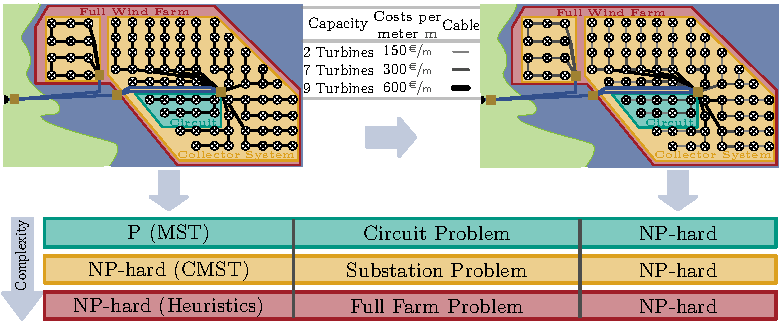
\includegraphics[page=1]{relatedwork/figures/windfarm-overview.pdf}
    % 
    \caption[The complexity of wind farm cabling problems.]{%
    The wind farm topology consists typically of turbines~\tikzTurbine and
    substations~\tikzSubstation. The complexity of cabling a wind farm differs
    depending on the cost function. If we assume unit costs---meaning we have
    only one cable type~\tikzOneTransportCable available---then the problem is
    slightly easier to solve (see left side) than when allowing multiple cable
    types~\tikzTransportCable (see right side). The different cable types are
    shown in the table. The complexity of the problem also increases dependent
    on the problem layers. The easiest layer is the~\glslongform{cp} (\gls{cp}),
    followed by the~\glslongform{sp} (\gls{sp}) and~\glslongform{ffp}
    (\gls{ffp}). }%
    % 
    \label{ch:related-work:sec:wind-farm-cabling:fig:windfarm-overview}
    % 
\end{figure}
% 
The amount of renewable energy producers started to increase significantly a few
years ago. However, there is not a lot of research done in the field of wind
farm planning. From an algorithmic point of view and using just a single cable
type, the~\glslongform{cp}~(\gls{cp}) can be solved using a~\acrlong{mst}
(\gls{mst}) algorithm~\parencite{Held1971, Gabow1986}, whereas
the~\glslongform{sp}~(\gls{sp}) can be solved
using~\acrlong{cmst}~(\gls{cmst})~\parencite{Vos09}. However,
\gls{cmst} is already~\NP-hard, but approximation algorithms and heuristics
exist for this type of problem~\parencite{5388449, Mar67, Vos09}. This is
visualized
in~\cref{ch:related-work:sec:wind-farm-cabling:fig:windfarm-overview}. We are
interested in the layout problem using multiple cable types with different
capacities and costs per meter, which is already \NP-hard for two cable types in
the~\glslongform{cp}. Using brute force for~$\fmagnitude{\cabletypes}$ different
cable types and~$\fmagnitude{\glssymbol{edges}}$ possible interconnections would
mean that there are~$\fmagnitude{\cabletypes}^{\fmagnitude{\glssymbol{edges}} }$
possible combinations to compute. However, to compute cabling layouts with
multiple cable types some work is done in the area of cluster-based,
\gls{mst}-based and genetic algorithms. \textcite{5740480} used
the~\glslongform{qt}~(\gls{qt}) Clustering algorithm to group the turbines into
collector systems or even groups within a collector system. They
evaluate---based on reliability, power losses and cabling costs---three
different layouts namely the radial, cluster-based, and mixed layout.

If the wind farm planning does not consider the cabling of turbines, but the
connection of entire offshore wind farms among themselves and to the mainland,
then the clustering approach based
on~$k$-mean~\parencite{Kanungo:2002:EKC:628329.628801} from~\textcite{Sve13}
tries to model and propose an algorithm for that kind of problem by taking
investment costs and operational costs with different stakeholders into account.

A more general attempt---not using clustering, but a~\gls{mst}-based
approach---was given by~\textcite{berzan}. It solves the circuit problem for
multiple cable types. 

In contrast, evolutionary algorithms present a very promising approach to solve
complex, multi-variable and multi-objective optimization problems with many
design variables (see~\cref{ch:wfcp}). Within evolutionary algorithms,
a~\acrlong{ga}~(\gls{ga}) is usually applied to problems with huge solution
space and discrete variables. There are~\gls{ga} approaches introducing
different encodings and solution methods for electrical systems integrating
different electrical components to be optimized such as type of turbine and
substation~\parencite{citeulike:7362179, 4957255, 5348118, 4152877, 6007042}.

A different modeling approach was proposed
by~\textcite{doi:10.3138/infor.50.2.095} including unsplittable electrical flows
into the~\acrlong{milp}~(\gls{milp}) for the wind farm design problem, which
forbids to split the incoming power from one cable.%4218649

In general, the cabling problem has a lot in common with transportation of
goods, where the cost of laying a cable does not necessarily depend on the
actual amount of power it transports. If the maximum power exceeds the capacity
(thermal limit) of a cable, a different and more expensive cable is deployed.
This raises the costs in a non-convex manner and makes it
\NP-hard~\parencite{20084889}. In transportation of goods, trucks and goods are
an analogous example of cables and power, respectively. Heuristical approaches
to solve the problem in logistics are Tabu Search~\parencite{Glover1999}, Ant
Colony Optimization~\parencite{Dorigo2001} and~\acrlong{sa}
(\gls{sa})~\parencite{Osman1996}. \citeauthor{20084889} solved
the~\acrlong{mcnd} (\gls{mcnd}) Problem in the field of logistics with
a~\gls{sa} approach. This algorithm serves as basis for our algorithm and
is improved for the wind farm cabling problem.

In contrast to the~\gls{ga} approaches, we are not interested in solving
the configuration, but the physical layout. Furthermore, the choice of
the~\gls{ga}'s cost function is debatable, since integrating the throughput
of a farm might be also important. Our model omits unsplittable flows, since it
increases the complexity of the problem without bringing an additional benefit
and distorts the electrical reality.

Most of the papers evaluate their algorithms on a small instance or on a small
set of benchmark data. Especially for evolutionary algorithms, this can lead to
a falsification of the results, since the configuration of the algorithm is
improved with regards to one specific data set, but might perform poorly on
others. Thus, we generate a test data benchmark set on which we perform our
simulations to avoid such effects and give a more general statement.